% Options for packages loaded elsewhere
\PassOptionsToPackage{unicode}{hyperref}
\PassOptionsToPackage{hyphens}{url}
%
\documentclass[
]{article}
\usepackage{amsmath,amssymb}
\usepackage{iftex}
\ifPDFTeX
  \usepackage[T1]{fontenc}
  \usepackage[utf8]{inputenc}
  \usepackage{textcomp} % provide euro and other symbols
\else % if luatex or xetex
  \usepackage{unicode-math} % this also loads fontspec
  \defaultfontfeatures{Scale=MatchLowercase}
  \defaultfontfeatures[\rmfamily]{Ligatures=TeX,Scale=1}
\fi
\usepackage{lmodern}
\ifPDFTeX\else
  % xetex/luatex font selection
\fi
% Use upquote if available, for straight quotes in verbatim environments
\IfFileExists{upquote.sty}{\usepackage{upquote}}{}
\IfFileExists{microtype.sty}{% use microtype if available
  \usepackage[]{microtype}
  \UseMicrotypeSet[protrusion]{basicmath} % disable protrusion for tt fonts
}{}
\makeatletter
\@ifundefined{KOMAClassName}{% if non-KOMA class
  \IfFileExists{parskip.sty}{%
    \usepackage{parskip}
  }{% else
    \setlength{\parindent}{0pt}
    \setlength{\parskip}{6pt plus 2pt minus 1pt}}
}{% if KOMA class
  \KOMAoptions{parskip=half}}
\makeatother
\usepackage{xcolor}
\usepackage[margin=1in]{geometry}
\usepackage{color}
\usepackage{fancyvrb}
\newcommand{\VerbBar}{|}
\newcommand{\VERB}{\Verb[commandchars=\\\{\}]}
\DefineVerbatimEnvironment{Highlighting}{Verbatim}{commandchars=\\\{\}}
% Add ',fontsize=\small' for more characters per line
\usepackage{framed}
\definecolor{shadecolor}{RGB}{248,248,248}
\newenvironment{Shaded}{\begin{snugshade}}{\end{snugshade}}
\newcommand{\AlertTok}[1]{\textcolor[rgb]{0.94,0.16,0.16}{#1}}
\newcommand{\AnnotationTok}[1]{\textcolor[rgb]{0.56,0.35,0.01}{\textbf{\textit{#1}}}}
\newcommand{\AttributeTok}[1]{\textcolor[rgb]{0.13,0.29,0.53}{#1}}
\newcommand{\BaseNTok}[1]{\textcolor[rgb]{0.00,0.00,0.81}{#1}}
\newcommand{\BuiltInTok}[1]{#1}
\newcommand{\CharTok}[1]{\textcolor[rgb]{0.31,0.60,0.02}{#1}}
\newcommand{\CommentTok}[1]{\textcolor[rgb]{0.56,0.35,0.01}{\textit{#1}}}
\newcommand{\CommentVarTok}[1]{\textcolor[rgb]{0.56,0.35,0.01}{\textbf{\textit{#1}}}}
\newcommand{\ConstantTok}[1]{\textcolor[rgb]{0.56,0.35,0.01}{#1}}
\newcommand{\ControlFlowTok}[1]{\textcolor[rgb]{0.13,0.29,0.53}{\textbf{#1}}}
\newcommand{\DataTypeTok}[1]{\textcolor[rgb]{0.13,0.29,0.53}{#1}}
\newcommand{\DecValTok}[1]{\textcolor[rgb]{0.00,0.00,0.81}{#1}}
\newcommand{\DocumentationTok}[1]{\textcolor[rgb]{0.56,0.35,0.01}{\textbf{\textit{#1}}}}
\newcommand{\ErrorTok}[1]{\textcolor[rgb]{0.64,0.00,0.00}{\textbf{#1}}}
\newcommand{\ExtensionTok}[1]{#1}
\newcommand{\FloatTok}[1]{\textcolor[rgb]{0.00,0.00,0.81}{#1}}
\newcommand{\FunctionTok}[1]{\textcolor[rgb]{0.13,0.29,0.53}{\textbf{#1}}}
\newcommand{\ImportTok}[1]{#1}
\newcommand{\InformationTok}[1]{\textcolor[rgb]{0.56,0.35,0.01}{\textbf{\textit{#1}}}}
\newcommand{\KeywordTok}[1]{\textcolor[rgb]{0.13,0.29,0.53}{\textbf{#1}}}
\newcommand{\NormalTok}[1]{#1}
\newcommand{\OperatorTok}[1]{\textcolor[rgb]{0.81,0.36,0.00}{\textbf{#1}}}
\newcommand{\OtherTok}[1]{\textcolor[rgb]{0.56,0.35,0.01}{#1}}
\newcommand{\PreprocessorTok}[1]{\textcolor[rgb]{0.56,0.35,0.01}{\textit{#1}}}
\newcommand{\RegionMarkerTok}[1]{#1}
\newcommand{\SpecialCharTok}[1]{\textcolor[rgb]{0.81,0.36,0.00}{\textbf{#1}}}
\newcommand{\SpecialStringTok}[1]{\textcolor[rgb]{0.31,0.60,0.02}{#1}}
\newcommand{\StringTok}[1]{\textcolor[rgb]{0.31,0.60,0.02}{#1}}
\newcommand{\VariableTok}[1]{\textcolor[rgb]{0.00,0.00,0.00}{#1}}
\newcommand{\VerbatimStringTok}[1]{\textcolor[rgb]{0.31,0.60,0.02}{#1}}
\newcommand{\WarningTok}[1]{\textcolor[rgb]{0.56,0.35,0.01}{\textbf{\textit{#1}}}}
\usepackage{graphicx}
\makeatletter
\def\maxwidth{\ifdim\Gin@nat@width>\linewidth\linewidth\else\Gin@nat@width\fi}
\def\maxheight{\ifdim\Gin@nat@height>\textheight\textheight\else\Gin@nat@height\fi}
\makeatother
% Scale images if necessary, so that they will not overflow the page
% margins by default, and it is still possible to overwrite the defaults
% using explicit options in \includegraphics[width, height, ...]{}
\setkeys{Gin}{width=\maxwidth,height=\maxheight,keepaspectratio}
% Set default figure placement to htbp
\makeatletter
\def\fps@figure{htbp}
\makeatother
\setlength{\emergencystretch}{3em} % prevent overfull lines
\providecommand{\tightlist}{%
  \setlength{\itemsep}{0pt}\setlength{\parskip}{0pt}}
\setcounter{secnumdepth}{-\maxdimen} % remove section numbering
\ifLuaTeX
  \usepackage{selnolig}  % disable illegal ligatures
\fi
\IfFileExists{bookmark.sty}{\usepackage{bookmark}}{\usepackage{hyperref}}
\IfFileExists{xurl.sty}{\usepackage{xurl}}{} % add URL line breaks if available
\urlstyle{same}
\hypersetup{
  pdftitle={Lab\_10},
  pdfauthor={izd3},
  hidelinks,
  pdfcreator={LaTeX via pandoc}}

\title{Lab\_10}
\author{izd3}
\date{}

\begin{document}
\maketitle

Use only commands \& functions that are shown in the indicated chapter
or prior chapters.

\newpage

\hypertarget{problem-01---chapter-39-exercise-1a}{%
\subsection{Problem \#01 - Chapter 39 Exercise
\#1A}\label{problem-01---chapter-39-exercise-1a}}

\begin{Shaded}
\begin{Highlighting}[]
\CommentTok{\# Show your work here}
\FunctionTok{library}\NormalTok{(stringr)}
\end{Highlighting}
\end{Shaded}

\begin{verbatim}
## Warning: package 'stringr' was built under R version 4.2.3
\end{verbatim}

\begin{Shaded}
\begin{Highlighting}[]
\NormalTok{senlen}\OtherTok{\textless{}{-}}\FunctionTok{str\_subset}\NormalTok{(}\AttributeTok{string =}\NormalTok{ sentences,}\AttributeTok{pattern =} \StringTok{\textquotesingle{}the\textquotesingle{}}\NormalTok{)}
\FunctionTok{head}\NormalTok{(senlen,}\AttributeTok{n=}\DecValTok{10}\NormalTok{)}
\end{Highlighting}
\end{Shaded}

\begin{verbatim}
##  [1] "The birch canoe slid on the smooth planks."       
##  [2] "Glue the sheet to the dark blue background."      
##  [3] "It's easy to tell the depth of a well."           
##  [4] "The box was thrown beside the parked truck."      
##  [5] "The boy was there when the sun rose."             
##  [6] "The source of the huge river is the clear spring."
##  [7] "Kick the ball straight and follow through."       
##  [8] "Help the woman get back to her feet."             
##  [9] "A pot of tea helps to pass the evening."          
## [10] "The soft cushion broke the man's fall."
\end{verbatim}

\begin{Shaded}
\begin{Highlighting}[]
\FunctionTok{length}\NormalTok{(senlen)}
\end{Highlighting}
\end{Shaded}

\begin{verbatim}
## [1] 408
\end{verbatim}

\newpage

\hypertarget{problem-02---chapter-40-exercise-1a}{%
\subsection{Problem \#02 - Chapter 40 Exercise
\#1A}\label{problem-02---chapter-40-exercise-1a}}

\begin{Shaded}
\begin{Highlighting}[]
\CommentTok{\# Show your work here}
\NormalTok{senlen}\OtherTok{\textless{}{-}}\FunctionTok{str\_subset}\NormalTok{(}\AttributeTok{string =}\NormalTok{ sentences,}\AttributeTok{pattern=}\StringTok{\textquotesingle{}ch[aeiou]\textquotesingle{}}\NormalTok{)}
\FunctionTok{head}\NormalTok{(senlen,}\AttributeTok{n=}\DecValTok{10}\NormalTok{)}
\end{Highlighting}
\end{Shaded}

\begin{verbatim}
##  [1] "These days a chicken leg is a rare dish."      
##  [2] "The hogs were fed chopped corn and garbage."   
##  [3] "Mesh wire keeps chicks inside."                
##  [4] "The set of china hit the floor with a crash."  
##  [5] "The ripe taste of cheese improves with age."   
##  [6] "Bring your problems to the wise chief."        
##  [7] "Write a fond note to the friend you cherish."  
##  [8] "The jacket hung on the back of the wide chair."
##  [9] "The child almost hurt the small dog."          
## [10] "A young child should not suffer fright."
\end{verbatim}

\begin{Shaded}
\begin{Highlighting}[]
\FunctionTok{length}\NormalTok{(senlen)}
\end{Highlighting}
\end{Shaded}

\begin{verbatim}
## [1] 51
\end{verbatim}

\newpage

\hypertarget{problem-03---chapter-38-exercise-2a}{%
\subsection{Problem \#03 - Chapter 38 Exercise
2A}\label{problem-03---chapter-38-exercise-2a}}

\begin{Shaded}
\begin{Highlighting}[]
\CommentTok{\# Show your work here}
\FunctionTok{library}\NormalTok{(lubridate)}
\end{Highlighting}
\end{Shaded}

\begin{verbatim}
## Warning: package 'lubridate' was built under R version 4.2.3
\end{verbatim}

\begin{verbatim}
## 
## Attaching package: 'lubridate'
\end{verbatim}

\begin{verbatim}
## The following objects are masked from 'package:base':
## 
##     date, intersect, setdiff, union
\end{verbatim}

\begin{Shaded}
\begin{Highlighting}[]
\NormalTok{Dates002.tib}\SpecialCharTok{$}\NormalTok{dataData}\OtherTok{=}\FunctionTok{make\_date}\NormalTok{(}\AttributeTok{year=}\NormalTok{Dates002.tib}\SpecialCharTok{$}\NormalTok{A,}\AttributeTok{month =}\NormalTok{ Dates002.tib}\SpecialCharTok{$}\NormalTok{B,}\AttributeTok{day =}\NormalTok{ Dates002.tib}\SpecialCharTok{$}\NormalTok{C)}
\NormalTok{Dates002.tib}
\end{Highlighting}
\end{Shaded}

\begin{verbatim}
## # A tibble: 10 x 4
##        A     B C     dataData  
##    <int> <int> <chr> <date>    
##  1  1926     6 07    1926-06-07
##  2  2008     9 05    2008-09-05
##  3  2012     8 05    2012-08-05
##  4  1985     6 24    1985-06-24
##  5  1917     9 18    1917-09-18
##  6  1990     2 24    1990-02-24
##  7  1939    11 21    1939-11-21
##  8  2002     7 27    2002-07-27
##  9  1997     6 01    1997-06-01
## 10  2012     8 18    2012-08-18
\end{verbatim}

\newpage

\hypertarget{problem-04---chapter-38-exercise-5b}{%
\subsection{Problem \#04 - Chapter 38 Exercise
\#5B}\label{problem-04---chapter-38-exercise-5b}}

\begin{Shaded}
\begin{Highlighting}[]
\CommentTok{\# Show your work here}
\FunctionTok{library}\NormalTok{(ggplot2)}
\end{Highlighting}
\end{Shaded}

\begin{verbatim}
## Warning: package 'ggplot2' was built under R version 4.2.3
\end{verbatim}

\begin{Shaded}
\begin{Highlighting}[]
\NormalTok{Dates006.tib}\SpecialCharTok{$}\NormalTok{dateData}\OtherTok{=}\FunctionTok{ydm}\NormalTok{(Dates006.tib}\SpecialCharTok{$}\NormalTok{dateData)}
\NormalTok{Dates006.tib}\SpecialCharTok{|\textgreater{}}
  \FunctionTok{ggplot}\NormalTok{(}\AttributeTok{mapping=}\FunctionTok{aes}\NormalTok{(}\AttributeTok{x=}\NormalTok{dateData,}\AttributeTok{y=}\NormalTok{soilent,}\AttributeTok{color=}\NormalTok{people))}\SpecialCharTok{+}\FunctionTok{geom\_line}\NormalTok{()}\SpecialCharTok{+}\FunctionTok{facet\_wrap}\NormalTok{(}\SpecialCharTok{\textasciitilde{}}\NormalTok{people)}\SpecialCharTok{+}
  \FunctionTok{scale\_x\_date}\NormalTok{(}\AttributeTok{breaks =} \FunctionTok{make\_date}\NormalTok{(}\AttributeTok{year=}\FunctionTok{c}\NormalTok{(}\DecValTok{1900}\NormalTok{,}\DecValTok{2000}\NormalTok{,}\DecValTok{2020}\NormalTok{)),}\AttributeTok{date\_labels =} \StringTok{\textquotesingle{}\%Y\textquotesingle{}}\NormalTok{)}
\end{Highlighting}
\end{Shaded}

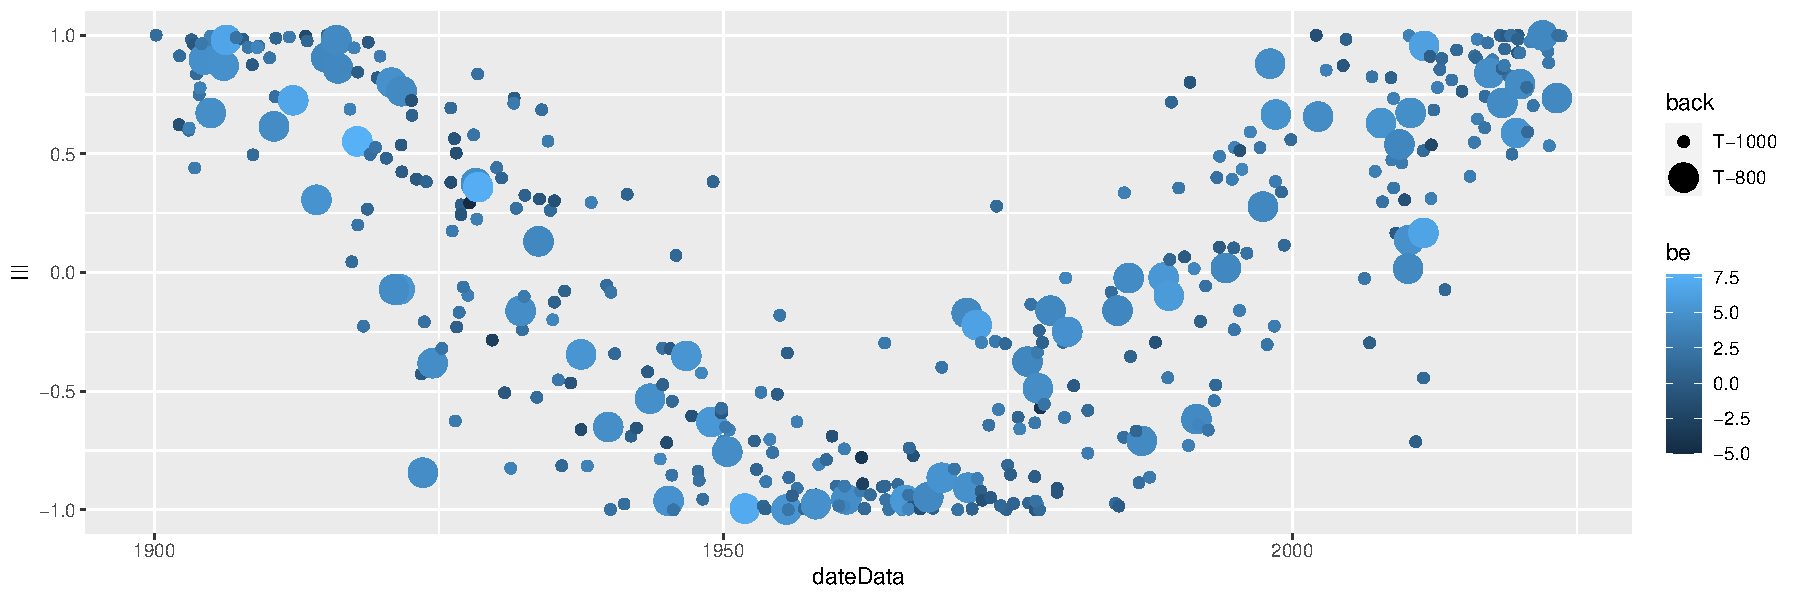
\includegraphics[height=300]{3040_Lab10_izd3_files/figure-latex/unnamed-chunk-4-1}

\end{document}
